\documentclass[dvisvgm,tikz]{standalone}
\usetikzlibrary{positioning,decorations.pathreplacing,calc}
\begin{document}
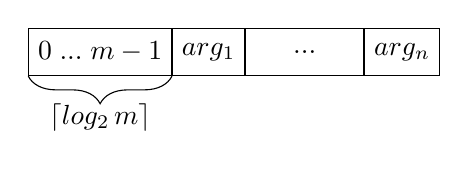
\begin{tikzpicture}
  \node[rectangle,draw,minimum height=0.6cm] (first) {$0 \; ... \; m - 1$};
  \node[rectangle,draw,minimum height=0.6cm,right=0cm of first] (second) {$arg_1$};
  \node[rectangle,draw,minimum height=0.6cm, minimum width=1.5cm,right=0cm of second] (third) {$...$};
  \node[rectangle,draw,minimum height=0.6cm,right=0cm of third] (fourth) {$arg_n$};
  \draw[decorate,decoration= {brace,mirror,amplitude=10pt}] (first.south west) -- (first.south east) node [midway,yshift=-15pt] {$\lceil log_2 \, m \rceil$};
\end{tikzpicture}
\end{document}

